\documentclass[tikz,border=8pt]{standalone}
\usetikzlibrary{positioning,arrows.meta,calc}
\begin{document}
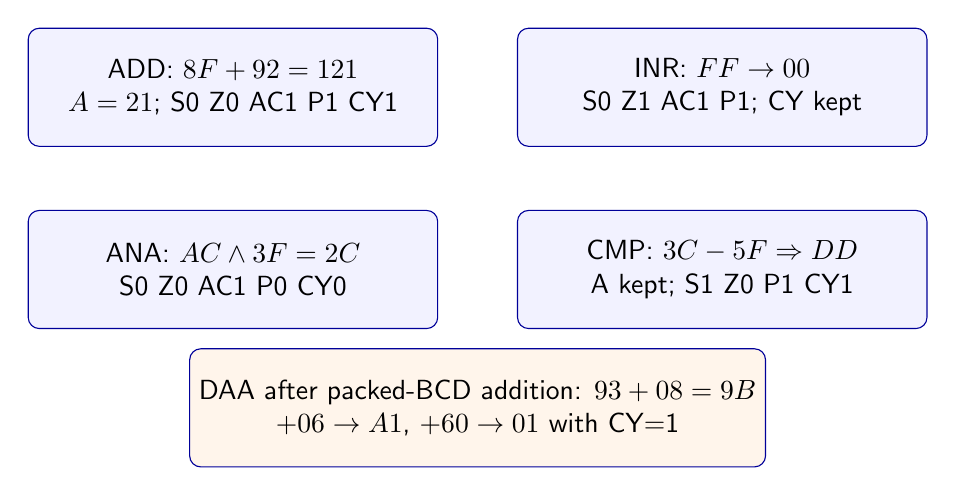
\begin{tikzpicture}[font=\sffamily,>=Latex,
box/.style={draw=blue!60!black,rounded corners,fill=blue!5,minimum width=52mm,minimum height=15mm,align=center},
arr/.style={->,thick,orange!80!black}]
\node[box] (add) {ADD: $8F+92=121$\\$A=21$; S0 Z0 AC1 P1 CY1};
\node[box,right=10mm of add] (inr) {INR: $FF\rightarrow00$\\S0 Z1 AC1 P1; CY kept};
\node[box,below=8mm of add] (ana) {ANA: $AC\land3F=2C$\\S0 Z0 AC1 P0 CY0};
\node[box,right=10mm of ana] (cmp) {CMP: $3C-5F\Rightarrow DD$\\A kept; S1 Z0 P1 CY1};
\node[box,below=10mm of {$(ana)!0.5!(cmp)$},minimum width=67mm,fill=orange!8] (daa) {DAA after packed-BCD addition: $93+08=9B$\\$+06\rightarrow A1$, $+60\rightarrow01$ with CY=1};
\end{tikzpicture}
\end{document}
